% This file was converted to LaTeX by Writer2LaTeX ver. 1.6
% see http://writer2latex.sourceforge.net for more info
\documentclass[letterpaper]{article}
\usepackage[latin1]{inputenc}
\usepackage{amsmath}
\usepackage{amssymb,amsfonts,textcomp}
\usepackage[T1]{fontenc}
\usepackage[english,french]{babel}
\usepackage{color}
\usepackage{array}
\usepackage{supertabular}
\usepackage{hhline}
\usepackage{hyperref}
\hypersetup{pdftex, colorlinks=true, linkcolor=blue, citecolor=blue, filecolor=blue, urlcolor=blue, pdftitle=, pdfauthor=, pdfsubject=, pdfkeywords=}
\usepackage[pdftex]{graphicx}
% Outline numbering
\setcounter{secnumdepth}{0}
\makeatletter
\newcommand\arraybslash{\let\\\@arraycr}
\makeatother
% Page layout (geometry)
\setlength\voffset{-1in}
\setlength\hoffset{-1in}
\setlength\topmargin{2cm}
\setlength\oddsidemargin{2cm}
\setlength\textheight{23.94cm}
\setlength\textwidth{17.59cm}
\setlength\footskip{0.0cm}
\setlength\headheight{0cm}
\setlength\headsep{0cm}
% Footnote rule
\setlength{\skip\footins}{0.119cm}
\renewcommand\footnoterule{\vspace*{-0.018cm}\setlength\leftskip{0pt}\setlength\rightskip{0pt plus 1fil}\noindent\textcolor{black}{\rule{0.25\columnwidth}{0.018cm}}\vspace*{0.101cm}}
% Pages styles
\makeatletter
\newcommand\ps@Standard{
  \renewcommand\@oddhead{}
  \renewcommand\@evenhead{}
  \renewcommand\@oddfoot{}
  \renewcommand\@evenfoot{}
  \renewcommand\thepage{\arabic{page}}
}
\makeatother
\pagestyle{Standard}
\setlength\tabcolsep{1mm}
\renewcommand\arraystretch{1.3}
% List styles
\newcommand\liststyleWWNumi{%
\renewcommand\theenumi{}
\renewcommand\theenumii{}
\renewcommand\theenumiii{}
\renewcommand\theenumiv{}
\renewcommand\labelenumi{\theenumi[200B?]}
\renewcommand\labelenumii{\theenumii[200B?]}
\renewcommand\labelenumiii{\theenumiii[200B?]}
\renewcommand\labelenumiv{\theenumiv[200B?]}
}
\newcommand\liststyleWWNumii{%
\renewcommand\theenumi{}
\renewcommand\theenumii{}
\renewcommand\theenumiii{}
\renewcommand\theenumiv{}
\renewcommand\labelenumi{\theenumi[200B?]}
\renewcommand\labelenumii{\theenumii[200B?]}
\renewcommand\labelenumiii{\theenumiii[200B?]}
\renewcommand\labelenumiv{\theenumiv[200B?]}
}
\newcommand\liststyleWWNumiii{%
\renewcommand\theenumi{\arabic{enumi}}
\renewcommand\theenumii{}
\renewcommand\theenumiii{}
\renewcommand\theenumiv{}
\renewcommand\labelenumi{\theenumi}
\renewcommand\labelenumii{\theenumii[200B?]}
\renewcommand\labelenumiii{\theenumiii[200B?]}
\renewcommand\labelenumiv{\theenumiv[200B?]}
}
\newcommand\liststyleWWNumiv{%
\renewcommand\theenumi{}
\renewcommand\theenumii{}
\renewcommand\theenumiii{}
\renewcommand\theenumiv{}
\renewcommand\labelenumi{\theenumi[200B?]}
\renewcommand\labelenumii{\theenumii[200B?]}
\renewcommand\labelenumiii{\theenumiii[200B?]}
\renewcommand\labelenumiv{\theenumiv[200B?]}
}
\newcommand\liststyleWWNumv{%
\renewcommand\theenumi{}
\renewcommand\theenumii{}
\renewcommand\theenumiii{}
\renewcommand\theenumiv{}
\renewcommand\labelenumi{\theenumi[200B?]}
\renewcommand\labelenumii{\theenumii[200B?]}
\renewcommand\labelenumiii{\theenumiii[200B?]}
\renewcommand\labelenumiv{\theenumiv[200B?]}
}
\newcommand\liststyleWWNumvi{%
\renewcommand\theenumi{}
\renewcommand\theenumii{}
\renewcommand\theenumiii{}
\renewcommand\theenumiv{}
\renewcommand\labelenumi{\theenumi[200B?]}
\renewcommand\labelenumii{\theenumii[200B?]}
\renewcommand\labelenumiii{\theenumiii[200B?]}
\renewcommand\labelenumiv{\theenumiv[200B?]}
}
\newcommand\liststyleWWNumvii{%
\renewcommand\theenumi{\arabic{enumi}}
\renewcommand\theenumii{}
\renewcommand\theenumiii{}
\renewcommand\theenumiv{}
\renewcommand\labelenumi{\theenumi}
\renewcommand\labelenumii{\theenumii[200B?]}
\renewcommand\labelenumiii{\theenumiii[200B?]}
\renewcommand\labelenumiv{\theenumiv[200B?]}
}
\newcommand\liststyleWWNumviii{%
\renewcommand\theenumi{\arabic{enumi}}
\renewcommand\theenumii{}
\renewcommand\theenumiii{}
\renewcommand\theenumiv{}
\renewcommand\labelenumi{\theenumi}
\renewcommand\labelenumii{\theenumii[200B?]}
\renewcommand\labelenumiii{\theenumiii[200B?]}
\renewcommand\labelenumiv{\theenumiv[200B?]}
}
\newcommand\liststyleWWNumix{%
\renewcommand\theenumi{\arabic{enumi}}
\renewcommand\theenumii{}
\renewcommand\theenumiii{}
\renewcommand\theenumiv{}
\renewcommand\labelenumi{\theenumi}
\renewcommand\labelenumii{\theenumii[200B?]}
\renewcommand\labelenumiii{\theenumiii[200B?]}
\renewcommand\labelenumiv{\theenumiv[200B?]}
}
\newcommand\liststyleWWNumx{%
\renewcommand\theenumi{}
\renewcommand\theenumii{}
\renewcommand\theenumiii{}
\renewcommand\theenumiv{}
\renewcommand\labelenumi{\theenumi[200B?]}
\renewcommand\labelenumii{\theenumii[200B?]}
\renewcommand\labelenumiii{\theenumiii[200B?]}
\renewcommand\labelenumiv{\theenumiv[200B?]}
}
\newcommand\liststyleWWNumxi{%
\renewcommand\theenumi{\arabic{enumi}}
\renewcommand\theenumii{}
\renewcommand\theenumiii{}
\renewcommand\theenumiv{}
\renewcommand\labelenumi{\theenumi}
\renewcommand\labelenumii{\theenumii[200B?]}
\renewcommand\labelenumiii{\theenumiii[200B?]}
\renewcommand\labelenumiv{\theenumiv[200B?]}
}
\newcommand\liststyleWWNumxii{%
\renewcommand\theenumi{\arabic{enumi}}
\renewcommand\theenumii{}
\renewcommand\theenumiii{}
\renewcommand\theenumiv{}
\renewcommand\labelenumi{\theenumi}
\renewcommand\labelenumii{\theenumii[200B?]}
\renewcommand\labelenumiii{\theenumiii[200B?]}
\renewcommand\labelenumiv{\theenumiv[200B?]}
}
\newcommand\liststyleWWNumxiii{%
\renewcommand\theenumi{}
\renewcommand\theenumii{}
\renewcommand\theenumiii{}
\renewcommand\theenumiv{}
\renewcommand\labelenumi{\theenumi[200B?]}
\renewcommand\labelenumii{\theenumii[200B?]}
\renewcommand\labelenumiii{\theenumiii[200B?]}
\renewcommand\labelenumiv{\theenumiv[200B?]}
}
\newcommand\liststyleWWNumxiv{%
\renewcommand\theenumi{\arabic{enumi}}
\renewcommand\theenumii{}
\renewcommand\theenumiii{}
\renewcommand\theenumiv{}
\renewcommand\labelenumi{\theenumi}
\renewcommand\labelenumii{\theenumii[200B?]}
\renewcommand\labelenumiii{\theenumiii[200B?]}
\renewcommand\labelenumiv{\theenumiv[200B?]}
}
\newcommand\liststyleWWNumxv{%
\renewcommand\theenumi{\arabic{enumi}}
\renewcommand\theenumii{}
\renewcommand\theenumiii{}
\renewcommand\theenumiv{}
\renewcommand\labelenumi{\theenumi}
\renewcommand\labelenumii{\theenumii[200B?]}
\renewcommand\labelenumiii{\theenumiii[200B?]}
\renewcommand\labelenumiv{\theenumiv[200B?]}
}
\newcommand\liststyleWWNumxvi{%
\renewcommand\theenumi{\arabic{enumi}}
\renewcommand\theenumii{}
\renewcommand\theenumiii{}
\renewcommand\theenumiv{}
\renewcommand\labelenumi{\theenumi}
\renewcommand\labelenumii{\theenumii[200B?]}
\renewcommand\labelenumiii{\theenumiii[200B?]}
\renewcommand\labelenumiv{\theenumiv[200B?]}
}
\newcommand\liststyleWWNumxvii{%
\renewcommand\theenumi{\arabic{enumi}}
\renewcommand\theenumii{}
\renewcommand\theenumiii{}
\renewcommand\theenumiv{}
\renewcommand\labelenumi{\theenumi}
\renewcommand\labelenumii{\theenumii[200B?]}
\renewcommand\labelenumiii{\theenumiii[200B?]}
\renewcommand\labelenumiv{\theenumiv[200B?]}
}
\newcommand\liststyleWWNumxviii{%
\renewcommand\theenumi{\arabic{enumi}}
\renewcommand\theenumii{}
\renewcommand\theenumiii{}
\renewcommand\theenumiv{}
\renewcommand\labelenumi{\theenumi}
\renewcommand\labelenumii{\theenumii[200B?]}
\renewcommand\labelenumiii{\theenumiii[200B?]}
\renewcommand\labelenumiv{\theenumiv[200B?]}
}
\newcommand\liststyleWWNumxix{%
\renewcommand\theenumi{\arabic{enumi}}
\renewcommand\theenumii{}
\renewcommand\theenumiii{}
\renewcommand\theenumiv{}
\renewcommand\labelenumi{\theenumi}
\renewcommand\labelenumii{\theenumii[200B?]}
\renewcommand\labelenumiii{\theenumiii[200B?]}
\renewcommand\labelenumiv{\theenumiv[200B?]}
}
\newcommand\liststyleWWNumxx{%
\renewcommand\theenumi{\arabic{enumi}}
\renewcommand\theenumii{}
\renewcommand\theenumiii{}
\renewcommand\theenumiv{}
\renewcommand\labelenumi{\theenumi}
\renewcommand\labelenumii{\theenumii[200B?]}
\renewcommand\labelenumiii{\theenumiii[200B?]}
\renewcommand\labelenumiv{\theenumiv[200B?]}
}
\newcommand\liststyleWWNumxxi{%
\renewcommand\theenumi{}
\renewcommand\theenumii{}
\renewcommand\theenumiii{}
\renewcommand\theenumiv{}
\renewcommand\labelenumi{\theenumi[200B?]}
\renewcommand\labelenumii{\theenumii[200B?]}
\renewcommand\labelenumiii{\theenumiii[200B?]}
\renewcommand\labelenumiv{\theenumiv[200B?]}
}
\newcommand\liststyleWWNumxxii{%
\renewcommand\theenumi{\arabic{enumi}}
\renewcommand\theenumii{}
\renewcommand\theenumiii{}
\renewcommand\theenumiv{}
\renewcommand\labelenumi{\theenumi}
\renewcommand\labelenumii{\theenumii[200B?]}
\renewcommand\labelenumiii{\theenumiii[200B?]}
\renewcommand\labelenumiv{\theenumiv[200B?]}
}
\newcommand\liststyleWWNumxxiii{%
\renewcommand\theenumi{\arabic{enumi}}
\renewcommand\theenumii{}
\renewcommand\theenumiii{}
\renewcommand\theenumiv{}
\renewcommand\labelenumi{\theenumi}
\renewcommand\labelenumii{\theenumii[200B?]}
\renewcommand\labelenumiii{\theenumiii[200B?]}
\renewcommand\labelenumiv{\theenumiv[200B?]}
}
\newcommand\liststyleWWNumxxiv{%
\renewcommand\theenumi{\arabic{enumi}}
\renewcommand\theenumii{}
\renewcommand\theenumiii{}
\renewcommand\theenumiv{}
\renewcommand\labelenumi{\theenumi}
\renewcommand\labelenumii{\theenumii[200B?]}
\renewcommand\labelenumiii{\theenumiii[200B?]}
\renewcommand\labelenumiv{\theenumiv[200B?]}
}
\title{}
\author{}
\date{2018-10-07}
\begin{document}
{\centering\color{black}
Dual-Fuel Diesel Electric
\par}

\begin{figure}
\centering

\includegraphics{SimuEngEnForme-img/SimuEngEnForme-img001.jpg}
\end{figure}
\begin{figure}
\centering
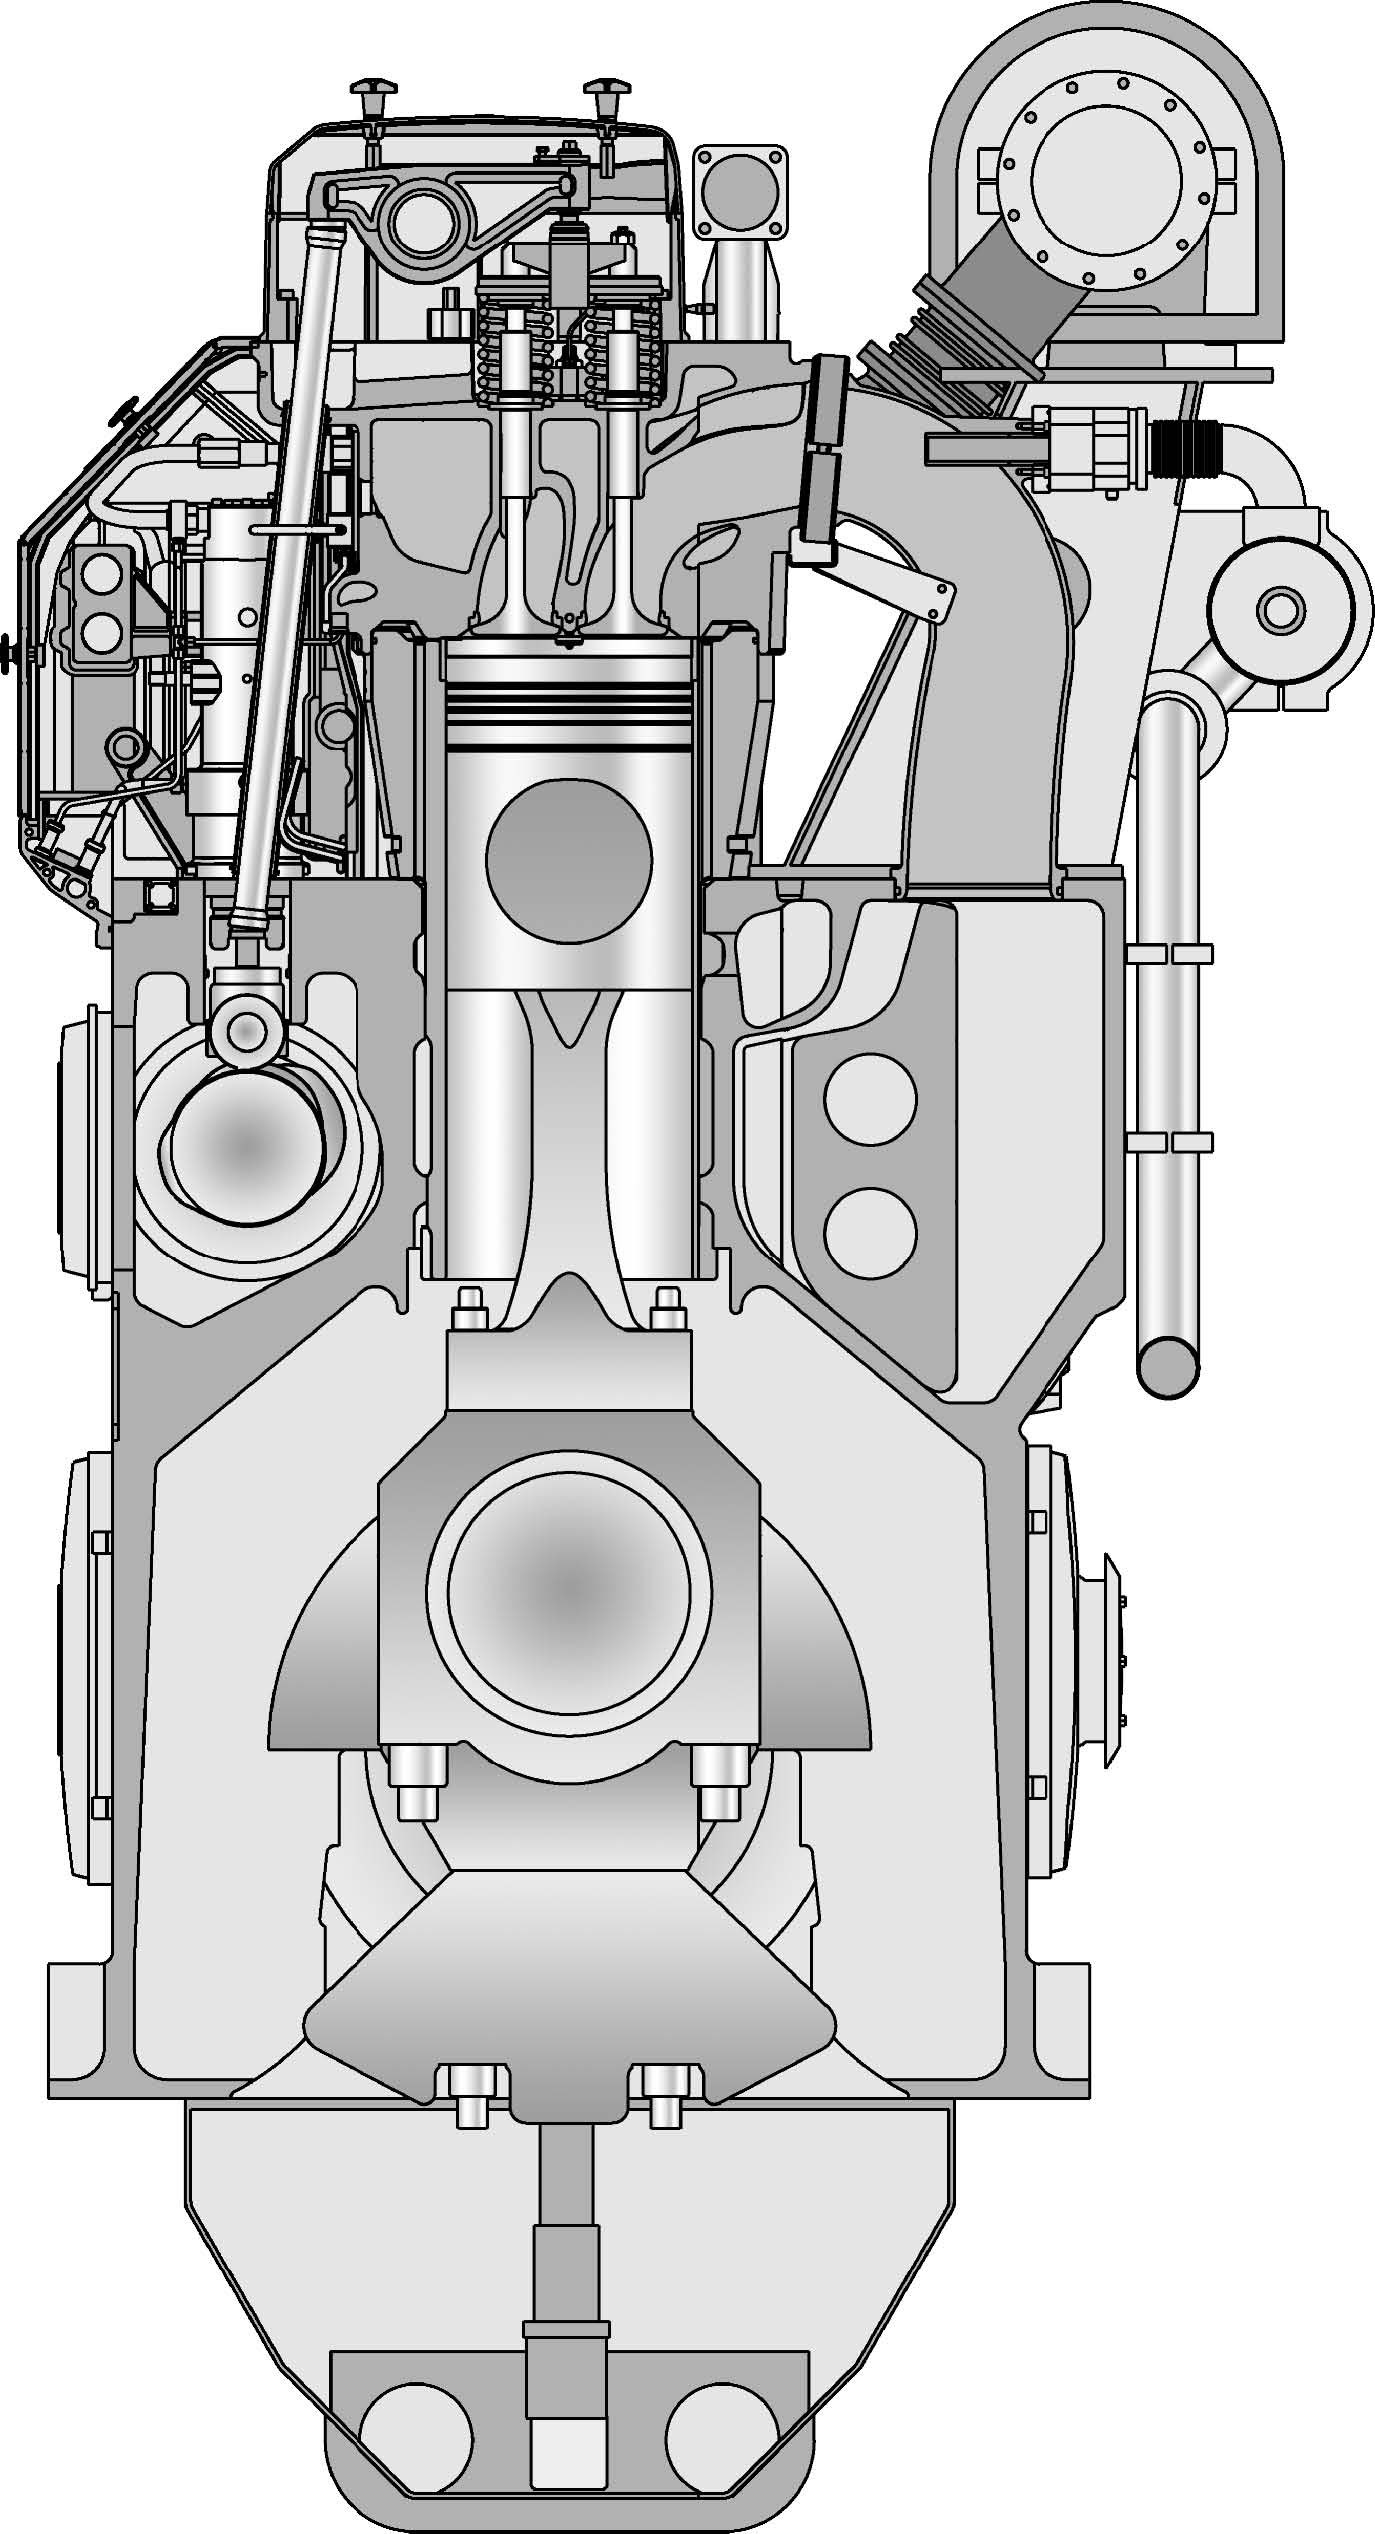
\includegraphics{SimuEngEnForme-img/SimuEngEnForme-img002.jpg}
\end{figure}
\begin{figure}
\centering
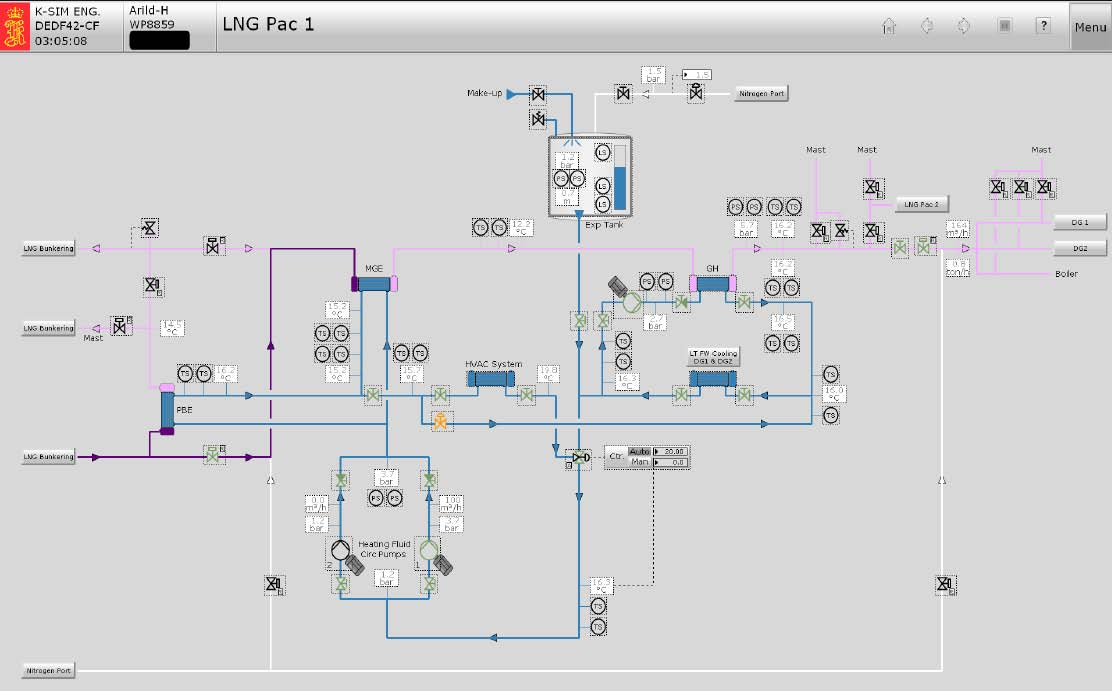
\includegraphics{SimuEngEnForme-img/SimuEngEnForme-img003.jpg}
\end{figure}
\begin{figure}
\centering
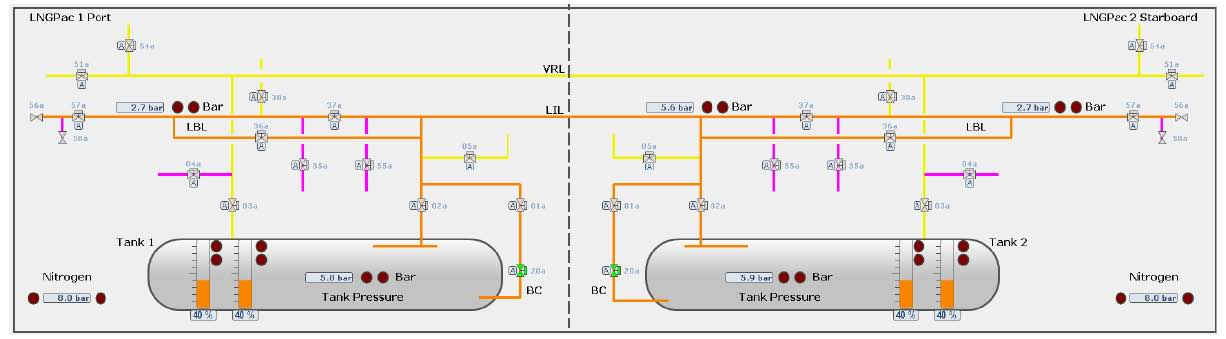
\includegraphics{SimuEngEnForme-img/SimuEngEnForme-img004.jpg}
\end{figure}
\begin{figure}
\centering
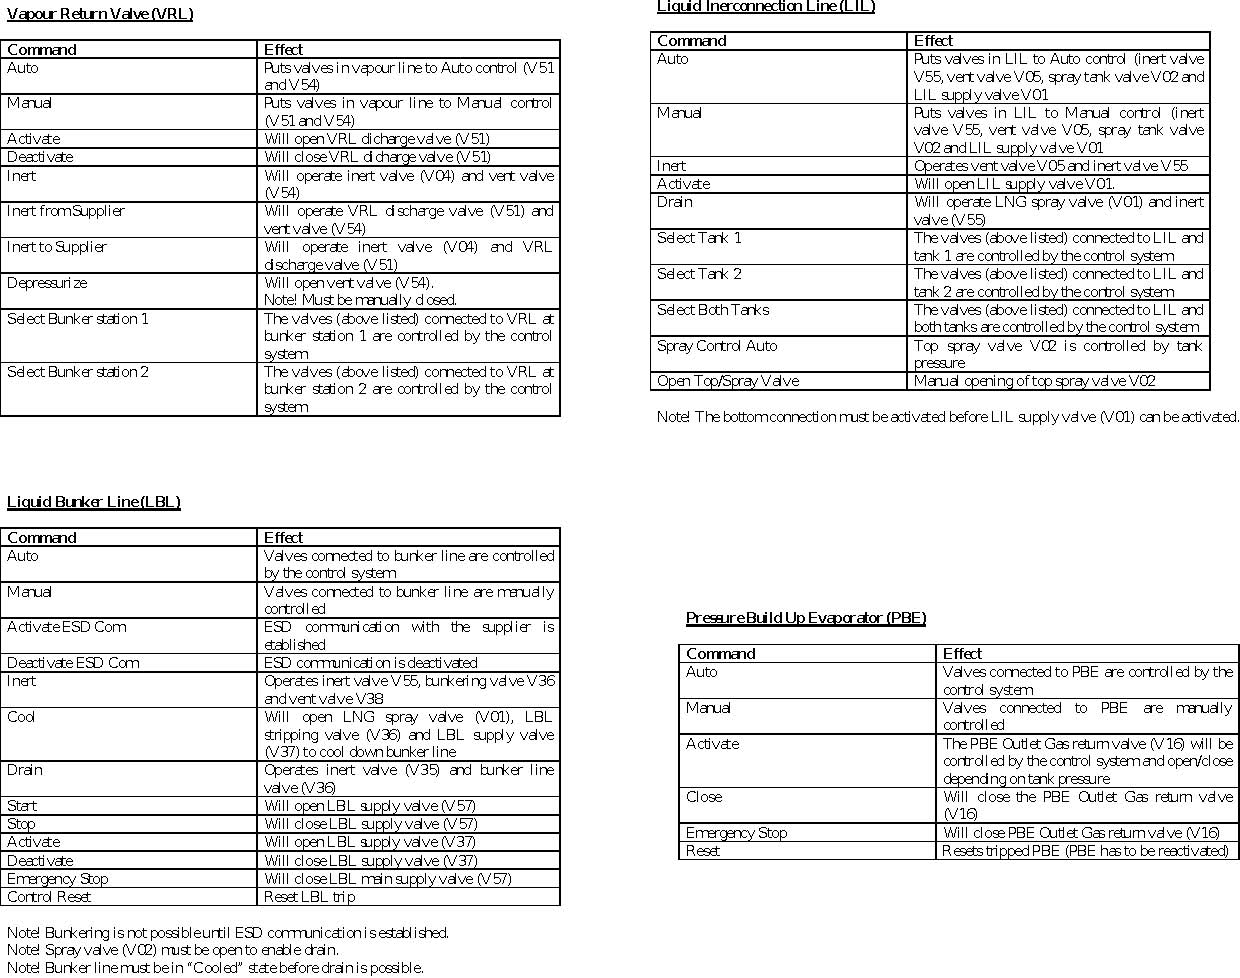
\includegraphics{SimuEngEnForme-img/SimuEngEnForme-img005.jpg}
\end{figure}
\begin{figure}
\centering
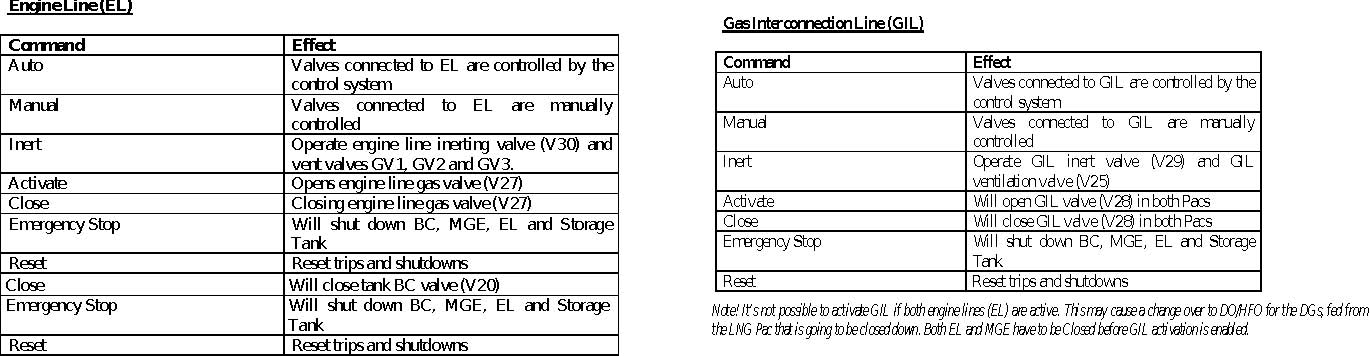
\includegraphics{SimuEngEnForme-img/SimuEngEnForme-img006.jpg}
\end{figure}
\begin{figure}
\centering
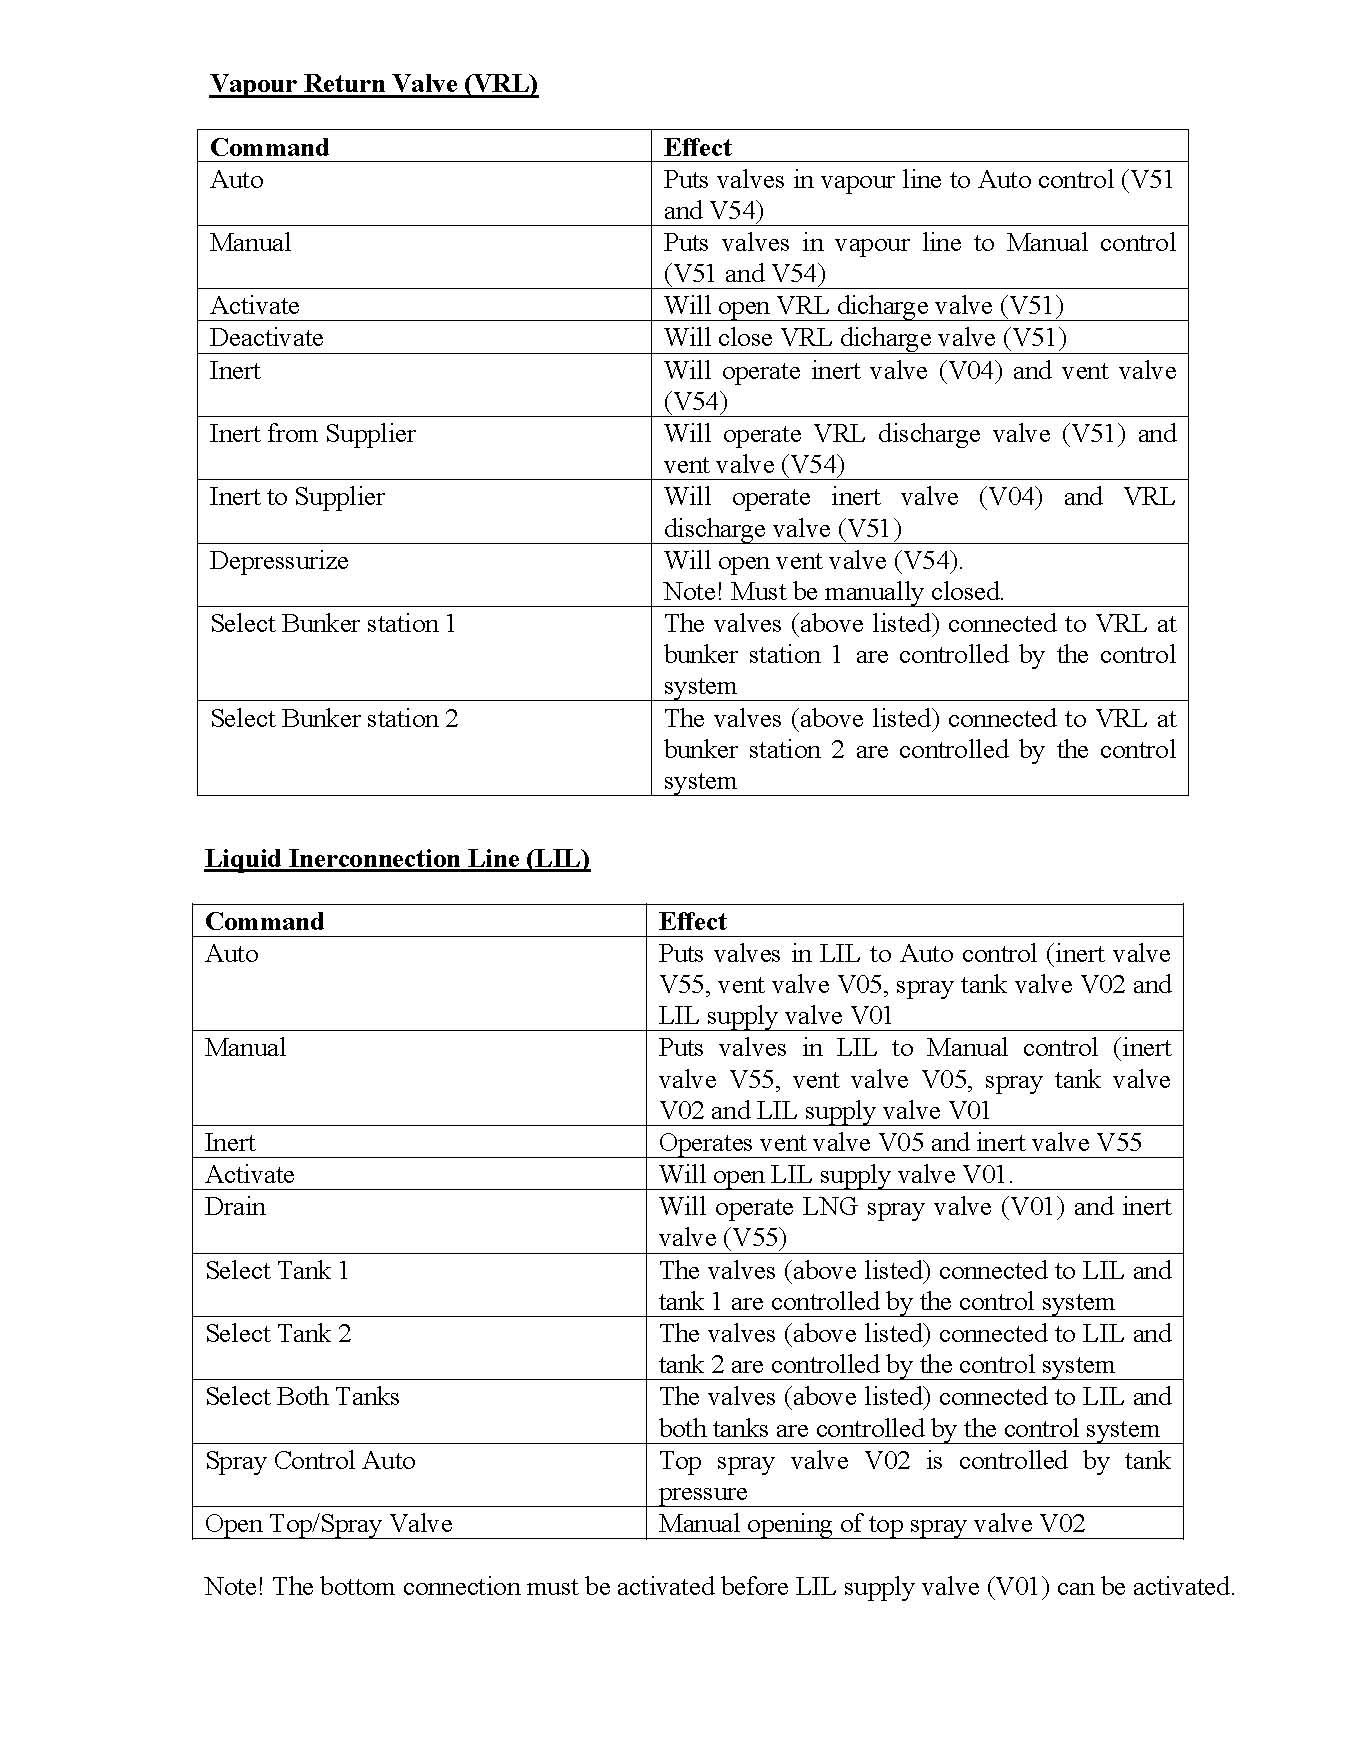
\includegraphics{SimuEngEnForme-img/SimuEngEnForme-img007.jpg}
\end{figure}
{\centering\color{black}
simulator type C
\par}

{\raggedleft\color{black}
Cyrille Reggio  2018
\par}

\section[1 Vessel data sheet]{1 Vessel data sheet }
\begin{flushleft}
\tablefirsthead{}
\tablehead{}
\tabletail{}
\tablelasttail{}
\begin{supertabular}{|m{6.979cm}|m{7.3830004cm}|}
\hline
{\color{black} Dead load capacity } &
\raggedleft\arraybslash{\color{black} 55,000 dwt }\\\hline
{\color{black} Length } &
\raggedleft\arraybslash{\color{black} 218 m }\\\hline
{\color{black} Width } &
\raggedleft\arraybslash{\color{black} 31,8 m }\\\hline
{\color{black} Maximum speed } &
\raggedleft\arraybslash{\color{black} 23 kt }\\\hline
{\color{black} Propulsive power } &
\raggedleft\arraybslash{\color{black} 21000 kW }\\\hline
{\color{black} Electric propulsion motors } &
\raggedleft\arraybslash{\color{black} 2 }\\\hline
{\color{black} DA } &
\raggedleft\arraybslash{\color{black} 4 x W�rtsil� 8L50DF (4 x 7,600 kW) }\\\hline
{\color{black} Main bus bar voltage } &
\raggedleft\arraybslash{\color{black} 6.6kV }\\\hline
{\color{black} Main bar} &
\raggedleft\arraybslash{\color{black} 4x400V }\\\hline
{\color{black} Bow thrusters } &
\raggedleft\arraybslash{\color{black} 2 }\\\hline
{\color{black} Stern thruster } &
\raggedleft\arraybslash{\color{black} 1 }\\\hline
\end{supertabular}
\end{flushleft}
{\color{black}
TABLE 1: Main Features }

{\color{black}
Dual Fuel Engines }

{\color{black}
 Wartsila 8L50DF }

\liststyleWWNumi
\begin{enumerate}
\item {\color{black}
{}- 7600 kW }
\item {\color{black}
{}- bore 500 mm }
\item {\color{black}
{}- 8 cylinders in line }
\item {\color{black}
{}- an air cooler }
\item {\color{black}
{}- Two turbo-souf[FB02?]antes }
\item {\color{black}
{}- 500 rpm }
\item {\color{black}
{}- gas mode / DO-HFO / backup (without pilot injection) }
\end{enumerate}
\section{2 Systems addressed }
{\centering\color{black}
The systems represented by the DFDE simulator are as follows: 
\par}

\liststyleWWNumii
\begin{enumerate}
\item \begin{enumerate}
\item {\color{black}
{}- IAS (Integrated Automation System) control system }
\item {\color{black}
{}- Alarm management, }
\item {\color{black}
{}- Electrical power management, }
\item {\color{black}
{}- Propulsion system. }
\item {\color{black}
{}- GE Dual Fuel management, }
\item {\color{black}
{}- LNG Operations Control System (Control System) }
\item {\color{black}
{}- LNG refuelling (truck, barge or pipe), }
\item {\color{black}
{}- Monitoring of operations, }
\item {\color{black}
{}- Gas quality, }
\item {\color{black}
{}- ESD system, }
\item {\color{black}
{}- LNG Storage }
\end{enumerate}
\item {\color{black}
{}- Gas operations before supplying the groups. }
\end{enumerate}
\section[3 Start{}-up ]{3 Start-up }
\liststyleWWNumiii
\begin{enumerate}
\item {\color{black}
Load the\textit{ DEDF42-CF} program, }
\item {\color{black}
Load the initial cold ship condition, }
\end{enumerate}
{\color{black}
Start the simulation with F1 then Home, the most common keyboard shortcuts are : }

\begin{flushleft}
\tablefirsthead{}
\tablehead{}
\tabletail{}
\tablelasttail{}
\begin{supertabular}{|m{1.931cm}|m{3.726cm}|}
\hline
{\color{black} Shortcut } &
{\color{black} Function }\\\hline
{\color{black} F1 } &
{\color{black} Run }\\\hline
{\color{black} F2 } &
{\color{black} Freeze }\\\hline
{\color{black} F3 } &
{\color{black} Stop }\\\hline
{\color{black} Shift+F6 } &
{\color{black} Initial condition }\\\hline
{\color{black} Home } &
{\color{black} Main page }\\\hline
{\color{black} Pg Up } &
{\color{black} Increase the page }\\\hline
{\color{black} Pg Down } &
{\color{black} Decrease the page }\\\hline
{\color{black} F12 } &
{\color{black} Ack buzzer }\\\hline
\end{supertabular}
\end{flushleft}
{\color{black}
TABLE 2: Keyboard shortcuts\textit{ }}

{\color{black}
\textit{Note that these shortcuts are also accessible via} Menu Operation }

\section[4 Cold ship start sequence ]{4 Cold ship start sequence }
\subsection{4.1 Overall process }
\begin{flushleft}
\tablefirsthead{}
\tablehead{}
\tabletail{}
\tablelasttail{}
\begin{supertabular}{|m{1.1259999cm}|m{11.784cm}|m{3.661cm}|}
\hline
\centering{\color{black} Stage } &
{\color{black} Action } &
{\color{black} Page }\\\hline
\centering{\color{black} 1 } &
{\color{black} Line up for MDO from MDO Service tank to DGs via the Emergency Fuel Feed Pump } &
{\color{black} (MD455 \& 460) }\\\hline
\centering{\color{black} 2 } &
{\color{black} Line up DG LO system } &
{\color{black} (md 305 \& 310) }\\\hline
\centering{\color{black} 3 } &
{\color{black} Line up DG cooling water system } &
{\color{black} (MD405-410) }\\\hline
\centering{\color{black} 4 } &
{\color{black} Start DG from local stand and connect it to main switchboard Note ! Connect electrical consumers to main
switchboard to achive heating from DGs. } &
{\color{black} (MD205-220) and MD105 }\\\hline
\centering{\color{black} 6 } &
{\color{black} Line up for normal fuel supply } &
{\color{black} (MD460) }\\\hline
\centering{\color{black} 7 } &
{\color{black} Prepare ventilation } &
\\\hline
\centering{\color{black} 8 } &
{\color{black} Prepare LNG supplier for bunkering (truck, ship or terminal) (MD480) } &
\\\hline
\centering{\color{black} 9 } &
{\color{black} Prepare vessel for bunkering } &
{\color{black} (MD510 \& 755) }\\\hline
\centering{\color{black} 10 } &
{\color{black} Line up for heating of LNG } &
{\color{black} (MD515) }\\\hline
\centering{\color{black} 11 } &
{\color{black} Prepare Gas Supply to DGs } &
\\\hline
\centering{\color{black} 12 } &
{\color{black} DO/HFO-Gas Change Over } &
\\\hline
\centering{\color{black} 13 } &
{\color{black} Line up and start up next Diesel Engine, start on Gas and connect to main switch board } &
\\\hline
\centering{\color{black} 14 } &
{\color{black} Prepare for start up of propulsion from engine control room } &
\\\hline
\centering{\color{black} 15 } &
{\color{black} Transfer control position to bridge } &
\\\hline
\centering{\color{black} 16 } &
{\color{black} Ready for Departure } &
\\\hline
\end{supertabular}
\end{flushleft}
{\color{black}
TABLE 3: Main steps }

\subsection[4.2 Procurement ]{4.2 Procurement }
\subsubsection{4.2.1 Equipment }
The vessel is equipped with two type C tanks for a total capacity of 400m3. The two tanks are maintained at 5 bar at a
temperature of -127${\circ}$C\textit{. The} ship is equipped with two nitrogen tanks for inerting, in particular of the
supply pipes, but also for pressurising the FWHT expansion box, the system is pressurised to 8bar. 

{\centering  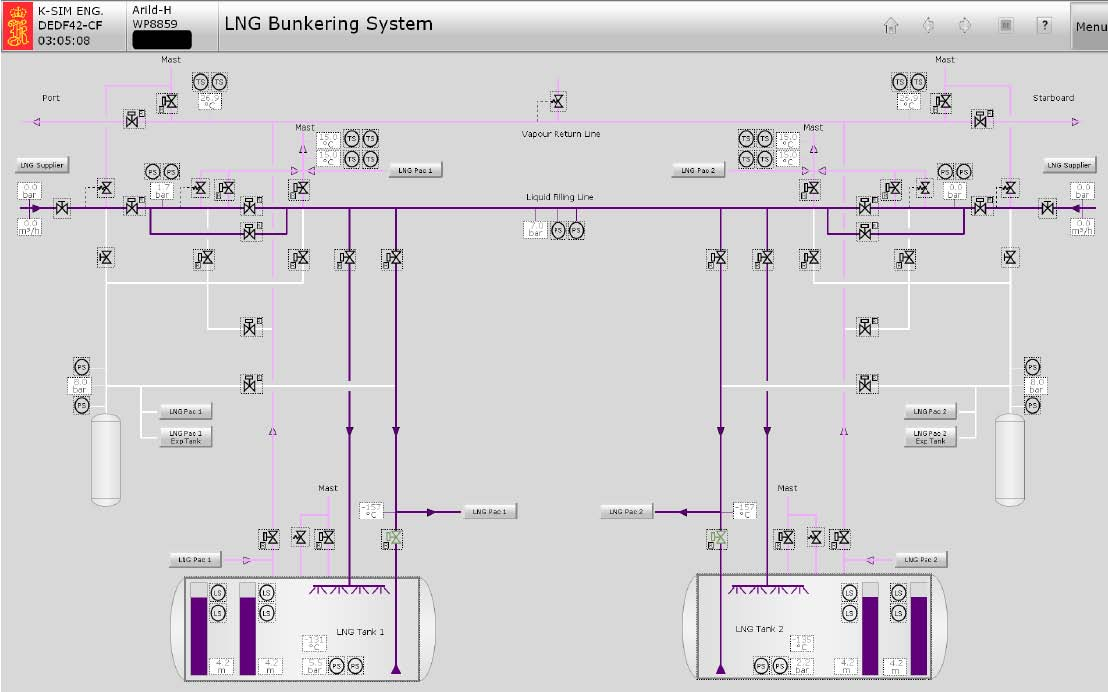
\includegraphics{SimuEngEnForme-img/SimuEngEnForme-img008.jpg} \par}
{\color{black}
FIGURE 1: LNG Bunkering System }

Each tank is equipped with a spray line that will allow: 

\liststyleWWNumiv
\begin{enumerate}
\item \ \ Refrigeration of the tank by vaporizing droplets during a cooling procedure, 
\item \ \ Tank pressure management during the supply operation, 
\end{enumerate}
The steam return lines and liquid lines are designed to be able to be in-terconnected. 

4.3 LNG supply 

The pressure delivered to the GVU during operation is 6.3barp to deliver the gas to 

2.3bar in the engine intake pipe, at a temperature of 34.1${\circ}$C. 

{\color{black}
FIGURE 2: LNG pac }

\subsection[4.4 Evaporators ]{4.4 Evaporators }
\subsubsection{4.4.1 Pressure Build Up Evaporator }
\textit{The Pressure Build Up Evaporator} allows the tank to be pressurized to 5.3bar, the gas is vaporized by the BT
fresh water circuit\textit{ (LT FW}) through a silicone gel (Syltherm) that acts as an interface between the ED and the
gas. The pressure is applied: 

\liststyleWWNumv
\begin{enumerate}
\item \ \ After the Initial Build Up operation, 
\item \ \ in operation a[FB01?]n to prevent the pressure drop in the vessel caused by the 
\end{enumerate}
gas consumption, the steam produced returns to the tank. 

\subsubsection{4.4.2 Main Gas Evaporator }
\textit{The Main Gas Evaporator is used to} manage the gas pressure delivered to the engine. It takes the gas in liquid
phase and vaporizes it. The pressure is regulated by regulating valves before and after the evaporators. 

\subsubsection{4.4.3 Gas Heater }
\textit{The Gas Heater provides the} [FB01?]nalisation temperature and pressure control for the engine. It has an
independent ED circuit to manage the [FB01?]nale phase of the heating system. The discharge pressure of the evaporators
(PBE, GVE) is regulated by the valve (V96) which redirects part of the flow to the Gas Heater. During free operation,
the set point of this valve is 40\%. 

{\color{black}
\textit{Note: the expansion tank has a nitrogen supply a[FB01?]n to maintain the tank pressure. It is also equipped with
a gas detection system; }}

\subsubsection{4.5 Safety valves }
The safety valves are located at different points in the circuit, their set pressure is 9bar. Their discharge is carried
out at the degassing mast. 

\section{5 Shutdown }
Several shutdown situations are planned: 

\liststyleWWNumvi
\begin{enumerate}
\item \item TAS (Tank Shutdown) : 
\item In case of failure of the\textit{ LNG PAC} circuit, the vents open a[FB01?]n to depressurize the pipework and the
closed automatic valves. A liquid phase gas return system sequenced to the tank ensures that only the minimum amount of
gas is vaporized. 
\item CB (Close Bunkering) : 
\item During the [FB01?]n supply operation, by closing the bunkering valves or in case of high level or high pressure in
the tank, 
\item BS (Bunkering Shutdown) : 
\item Supply valves if closed manually during operation cause a shutdown. 
\item ELS (Engine Line Shutdown) : In the event of an incident on the gas supply circuit, the inlet and outlet valves at
the MGE, and the interconnection valve are closed, the shutdown signal is sent to the GVU. 
\end{enumerate}
\subsection[5.1 Gas and ESD detection ]{5.1 Gas and ESD detection }
The detection is based on the detection of gas and oxygen. A pre-alarm and an alarm whose threshold can be
con[FB01?]gur� in the\textit{ Gas Detector Panel}. 

\section{6 Control System (LNG Monitor) }
The control system largely automates the procedures related to the gas circuit and allows the control and monitoring of
operations. 

\subsection{6.0.1 Control Box Command }
It allows operations on the fuel to be carried out and their progress to be monitored. 

{\color{black}
FIGURE 4: Disposition Storage tank }

The tables below illustrate each sequence automatically of the different elements of the circuit. 

{\centering
I
\par}

{\centering\color{black}
Diesel Alternator starting procedure Power supply
\par}

{\color{black}
Prerequisites The following circuits must be arranged: (Valves open, auxiliary pumps started) }

\liststyleWWNumvii
\begin{enumerate}
\item {\color{black}
EDBT }
\item {\color{black}
Oil }
\item {\color{black}
DO (the DO emergency pump runs on Emergency Fuel Feed Pump compressed air) }
\end{enumerate}
{\color{black}
\textit{Note: Compressed air is always available.} Before starting a group, it is necessary to switch it to DO/HFO mode,
be aware that in back-up mode (by default) it is impossible to switch to gas mode without stopping it. }

{\color{black}
Start-up:}

\liststyleWWNumviii
\begin{enumerate}
\item {\color{black}
Open the flap ([FB02?]ap), }
\item {\color{black}
Make an electric turn and then disengage the turning gear, }
\item {\color{black}
Make a Blow turn, }
\item {\color{black}
Go back to local, }
\item {\color{black}
Acknowledge alarms, }
\item {\color{black}
Switch to run mode on the selector switch, }
\item {\color{black}
Start and observe the temperature rise of the exhausts, }
\item {\color{black}
If the settings are correct, switch the group to remote. }
\end{enumerate}
{\color{black}
We can then arrange the power supply on the main bars and disposal of the consumers. }

\liststyleWWNumix
\begin{enumerate}
\item {\color{black}
Connect the main circuit breaker, }
\item {\color{black}
Supply the complete busbar system, }
\end{enumerate}
{\color{black}
14. Feed consumers. It is now possible to arrange the main and auxiliary pumps of the ED and oil circuits in automatic
mode. }

{\color{black}
Pass the DG1 in priority 1 / auto / alone on bus Stop the MDO air pump. }

{\color{black}
Attention: }

{\color{black}
The ED temperature regulation can only be switched automatically on the IAS. It is necessary: }

\liststyleWWNumx
\begin{enumerate}
\item {\color{black}
{}- Pass the three-way remote control valves through the circuit, }
\item {\color{black}
{}- Then on the IAS in the FW Cooling System page, pass the corresponding valves }
\end{enumerate}
{\color{black}
in a car. The valve then turns orange to indicate that it is regulating. }

{\centering
II
\par}

{\centering\color{black}
Procedure for supplying GNLC tanks at room temperature
\par}

{\color{black}
In this example we will use the truck and the supply will be made on the port tank. The following steps must be
followed: }

{\color{black}
Truck side preparations }

{\color{black}
A leak test of the liquid and vapour line valves must be carried out. }

\liststyleWWNumxi
\begin{enumerate}
\item {\color{black}
Inert the liquid and vapour lines, }
\item {\color{black}
Stop the inerting and check the absence of leaks, }
\item {\color{black}
Put the lines in the air, }
\item {\color{black}
Close the valves of the liquid and steam lines. }
\end{enumerate}
{\color{black}
When the ship is ready (full seal removed), connect the loading arm. Warn the board that an ESD test must be conducted.
}

{\color{black}
\textit{Note that the edge can inert the truck and the truck can inert the edge. }}

{\color{black}
Edge preparations }

{\color{black}
Operations will be conducted from the {\textquotedbl}LNG Monitor System{\textquotedbl} page. }

{\color{black}
Inertage }

\liststyleWWNumxii
\begin{enumerate}
\item {\color{black}
Open the flange on the ship side and connect the [FB02?]exible of the truck, }
\item {\color{black}
Installation of the water curtain, }

\begin{enumerate}
\item {\color{black}
3. Inerting with nitrogen, during this operation, the Inert command must be sent twice for : }
\item {\color{black}
(a) Depressurize }
\item {\color{black}
(b) Inerting }
\end{enumerate}
\end{enumerate}
{\color{black}
\textit{In inerting operations, be careful not to {\textquotedbl}activate{\textquotedbl}! }}

{\color{black}
The operations will be carried out in {\textquotedbl}automatic{\textquotedbl} mode, select {\textquotedbl}All in
auto{\textquotedbl}. Inerting is conducted from the tank to the connection. }

\liststyleWWNumxiii
\begin{enumerate}
\item {\color{black}
{}- Bottom Connection (BC) Inerting }
\item {\color{black}
{}- Inertage of Liquid Interconnection Line (LIL) }
\item {\color{black}
{}- Inertage of the Port Liquid Bunker Line (LBL) }
\end{enumerate}
\liststyleWWNumxiv
\begin{enumerate}
\item {\color{black}
Open (activate) Bottom Connection 1 (V20), }
\item {\color{black}
Open (activate) the Liquid Interconnection Line (select tank 1 / activate) (V01), }
\item {\color{black}
Open the Top Spray High Boom (LIL) (V02), }
\item {\color{black}
Activate the Liquid Bunker Line (V37), }
\item {\color{black}
Open the head valve (V57) manually }
\item {\color{black}
Activate and test the ESD (the LIL valve (V57) must close) }
\end{enumerate}
{\centering
III
\par}

{\color{black}
A leak test (Leak Test) must now be performed on the loading flange, for this purpose: }

\liststyleWWNumxv
\begin{enumerate}
\item {\color{black}
Pressurize the line between the truck and the head valve (V57) with nitrogen (8 bar), }
\item {\color{black}
Open the nitrogen supply valve and the valve (V58 MD510), }
\item {\color{black}
Close the supply valve and v�ri[FB01?]er the absence of leakage (pressure at 8 bar), }
\item {\color{black}
vent through the vent (V10 MD510), }
\item {\color{black}
close the vent. }
\end{enumerate}
{\color{black}
Cooling of tanks }

\liststyleWWNumxvi
\begin{enumerate}
\item {\color{black}
Open the manual isolation valve (V56 MD510) }
\item {\color{black}
Control the steam cooling by the liquid line of the low-flow truck (5 m3/h), select\textit{ VAPOUR} then\textit{ ON}.
The temperature }
\item {\color{black}
Start of the control box (V57) by the LBL, }
\item {\color{black}
Cold descent to -60${\circ}$Cdu pipework and tank, }
\item {\color{black}
Opening of the liquid line and progressive rise up to 400m3/h, }
\item {\color{black}
Vaporization (spray) in auto (LIL), lower the pressure set point (Setpoint Bunke-ring) to 1.0bar, this has the effect of
keeping the tank as cold as possible by playing on the vaporization. }
\end{enumerate}
{\color{black}
LNG supply begins }

{\centering\color{black}
If the back pressure increases in the tank, open the steam return line. 
\par}

{\color{black}
Finalization }

\liststyleWWNumxvii
\begin{enumerate}
\item {\color{black}
at 85\%, ask the truck to chase the liquid with steam (1 minute at 5 m3/h), }
\item {\color{black}
Stop the supply through the Control Box (Stop LBL) (V57), }
\item {\color{black}
Disable (V37) and purge the BL (V35, V36), for this purpose it is necessary to open on the spray of the (LBL), }
\item {\color{black}
inert the liquid line (inert LBL) (V55, V36, V38) (2 times), }
\item {\color{black}
purge the LIL through the spray line (V55) and inerter (V05) (twice), }
\item {\color{black}
Disconnect the flange, supply operation completed\textit{.}}
\end{enumerate}
{\centering
IV 
\par}

{\centering\color{black}
Cold tank GNLC supply procedure
\par}

{\color{black}
This procedure applies most of the time, in fact, if an LNG stub exists in the tank it is considered cold. }

\liststyleWWNumxviii
\begin{enumerate}
\item {\color{black}
Establish the connection with the terminal, as soon as the connection is established, the ESD is connected, }
\item {\color{black}
Test the ESD, (V57) }
\item {\color{black}
V�ri[FB01?]er the tightness of the connection, }
\item {\color{black}
Enable CB }
\item {\color{black}
Activate the LIL from the control box by activating: {\textquotedbl}tanks Activate{\textquotedbl}, }
\item {\color{black}
from the LBL control box select {\textquotedbl}cool{\textquotedbl} then {\textquotedbl}activate{\textquotedbl} and
en[FB01?]n {\textquotedbl}start{\textquotedbl} }
\end{enumerate}
{\color{black}
\textit{The manual valves must be correctly positioned to allow the controlled valve to be opened. }}

\liststyleWWNumxix
\begin{enumerate}
\item {\color{black}
Enable steam return (V03 and V51) }
\item {\color{black}
Open the barge or terminal side of the liquid and steam valve, wait until the pressure is 4.5bar, }
\item {\color{black}
Start the supply operation (from 50m3/h to 400m3/h\textit{) }}
\item {\color{black}
At 85\%, start reducing the liquid flow and ask the barge to open the vapor bunkering line a[FB01?]n to pressurize the
lines to push the liquid, }
\item {\color{black}
When there is no more liquid flow, wait 30sec to empty the lines and then stop the supply operation (STOP and deactivate
from the LBL control box), }
\item {\color{black}
Purge the LBL (drain), }
\item {\color{black}
Purge the LBL, }
\item {\color{black}
Inert LIL, }
\end{enumerate}
{\color{black}
15. Inerter LBL, It is now necessary to disconnect the [FB02?]exible: }

\liststyleWWNumxx
\begin{enumerate}
\item {\color{black}
Inert the edge with nitrogen via the (V58), }
\item {\color{black}
When the nitrogen pressure reaches 8bar, purge the liquid line to the barge, }
\item {\color{black}
Close the valve (V58), open the vent of the liquid line of the barge, }
\item {\color{black}
When pressure is zero, close the vent to the barge, }
\item {\color{black}
Close the liquid part on the barge side. }
\end{enumerate}
{\color{black}
A[FB01?]n not to send gas to the atmosphere when disconnecting, the HHT must be inert. }

\liststyleWWNumxxi
\begin{enumerate}
\item {\color{black}
{}- Inform the barge of the opening of the HHT vent, }
\item {\color{black}
{}- Manually set the HHT, }
\item {\color{black}
{}- Close the steam return (V03), }
\item {\color{black}
{}- Open on nitrogen (V04) to inert towards the barge, }
\item {\color{black}
{}- When the inerting is complete, close the valves and return the HHT to auto, }
\item {\color{black}
{}- Disable and inert the HHT from the control box, }
\item {\color{black}
{}- purges the HHT to the barge and when the pressure is zero, stop and isolate the inerting, }
\item {\color{black}
{}- When the [FB02?]exible is depressurized, close the manual supply valve (V56), }
\item {\color{black}
{}- Disconnect the [FB02?]exible and place the full flange, }
\item {\color{black}
{}- Purge the line by opening the valve (V56) and (V58) several times }
\item {\color{black}
{}- Inert by opening the valve (V10) }
\item \end{enumerate}
{\color{black}
End of the procurement operation. }

{\centering
V
\par}

{\centering\color{black}
Conversion from engines to gas 
\par}

{\color{black}
LNG provision }

{\color{black}
The heating system for the evaporators must be installed; }

\liststyleWWNumxxii
\begin{enumerate}
\item {\color{black}
V�ri[FB01?]er the level of the expansion box and place the expansion valve 1.5 bar of nitrogen, }
\item {\color{black}
Arrange the water circuit, regulation in automatic, }
\item {\color{black}
Arrange the HVAC air conditioning, }
\end{enumerate}
{\color{black}
4. Start the pumps. Arrangement of the gas supply to the engines. }

\liststyleWWNumxxiii
\begin{enumerate}
\item {\color{black}
Activate the CB, if it has been depressurized, it must first be inerted, }
\item {\color{black}
Activate the Pressure Build Evaporator the pressure set point must be 5bar, }
\item {\color{black}
Activate the Engine Line, }
\item {\color{black}
When the tank pressure is correct, activate the Main Gas Evaporator, the inerter }
\end{enumerate}
{\color{black}
if necessary, the Gas Interconnection Line connection can be activated, but you must nevertheless: }

{\color{black}
{}- Have an MGE in service, }

{\color{black}
{}- Have the other MGE stopped but pressurized. The gas is arranged. }

{\color{black}
Conversion from engines to gas }

\liststyleWWNumxxiv
\begin{enumerate}
\item {\color{black}
The engine compartment ventilation must be started and then switched to auto }
\item {\color{black}
The manual supply valve for the GVU (V051) must be installed, }
\item {\color{black}
The GVU control in auto, }
\end{enumerate}
{\color{black}
4. The Mode gas is available. It is possible to start directly with gas. }
\end{document}
